% Jacobian-lens trajectory summary: gemma-3-{270m,1b,4b,12b}-it
% Build:  tectonic slides/jlens_summary.tex
\documentclass[aspectratio=169,10pt]{beamer}

\usetheme{default}
\usecolortheme{dove}
\setbeamertemplate{navigation symbols}{}
\setbeamertemplate{footline}[frame number]
\setbeamercolor{frametitle}{fg=black}
\setbeamerfont{frametitle}{series=\bfseries}
\setbeamerfont{title}{series=\bfseries}
\setbeamertemplate{itemize items}[circle]

\usepackage{booktabs}
\usepackage{graphicx}
\usepackage{xcolor}
\usepackage[T1]{fontenc}

\graphicspath{{../figs/}{figs/}}

\definecolor{up}{RGB}{20,110,60}
\definecolor{down}{RGB}{170,40,40}
\newcommand{\good}[1]{\textcolor{up}{#1}}
\newcommand{\bad}[1]{\textcolor{down}{#1}}

\title{Jacobian-lens trajectories under medical SFT}
\subtitle{\texttt{gemma-3-\{270m,1b,4b,12b\}-it}}
\author{}
\date{\today}

\begin{document}

\begin{frame}
  \titlepage
  \vspace{-2em}
  \centering\small
  Full fine-tune on \texttt{mix\_default}, lr $1\mathrm{e}{-5}$, log-spaced
  checkpoints to step 4882

  \vspace{0.8em}
  {\footnotesize\bad{Draft --- findings 2 and 3 are held pending the 27b arm.}
  All behavioral numbers are on the \textbf{current} instrument
  (\texttt{rp}$=$\texttt{1.1}, self-hosted Kimi judge); nothing here is
  comparable to a version of this deck dated before 2026-08-05.}
\end{frame}

% ---------------------------------------------------------------- setup
\begin{frame}{Setup}
  \begin{itemize}
    \item \textbf{Four arms}, identical seed and data order:
      \texttt{gemma-3-\{270m,1b,4b,12b\}-it}, full FT,
      lr $1\mathrm{e}{-5}$, completion-only loss. A 27b arm is in flight.
    \item \textbf{Log-spaced checkpoints} $\{1,2,4,\dots,4096\}$ + final (4882).
      $t=0$ is the untouched base, prepended by the probe.
    \item \textbf{Lens refit per checkpoint} on a frozen 1000-sequence generic
      (non-medical) WikiText corpus, taken from \texttt{jlens}'s own
      \texttt{load\_wikitext\_prompts} --- the lens is a function of the weights.
    \item \textbf{Concordance} on the frozen 193-prompt probe set:
      50 \texttt{general} + 50 \texttt{medical} (hand-authored one-hop cloze,
      style-matched control pairs) + 93 \texttt{multihop} from
      \texttt{jlens}'s \texttt{lens-eval-multihop.json}.
    \item \textbf{Behavioral} trajectory in parallel: MedQA, MedMCQA, PubMedQA,
      reported as \emph{answered} accuracy with answer rate alongside.
      \textbf{Scored by an LLM judge}, not a regex --- see the instrument slide.
  \end{itemize}
  \vfill
  {\footnotesize All lens numbers below are the \textbf{mean over the last
  $n/5$ source layers} (the probe's \texttt{kl\_final} / \texttt{top1\_final}):
  3 layers at 270m, 5 at 1b, 6 at 4b, 9 at 12b. Where the single final layer
  disagrees, it is called out explicitly --- see the read-out caveat.
  Coverage: 14 / 15 / 14 / 14 lens points (270m / 1b / 4b / 12b) --- all four
  complete. \textbf{Behavioral: all four arms are judge-scored, complete, and on
  one instrument} (14 / 15 / 14 / 14 points incl.\ $t{=}0$), so cross-size
  behavioral comparison is legitimate for the first time in this deck.}
\end{frame}

% ---------------------------------------------------------------- probe step
\begin{frame}{The probe step in detail}
  \small
  Runs in \texttt{.venv-jlens} (\texttt{transformers} 5.14.1 + \texttt{jlens}
  @ \texttt{581d398}) --- a second env, because the training pin 4.53.2 is
  hard-incompatible. Imports nothing from \texttt{gemma\_med}.

  \vspace{0.15em}
  \begin{columns}[T]
    \begin{column}{0.55\textwidth}
      \textbf{Per checkpoint} (base prepended as step 0, then
      \texttt{checkpoint-*}):
      \begin{enumerate}\setlength{\itemsep}{0em}
        \item \textbf{Load} $\rightarrow$ \texttt{jlens.from\_hf(hf, tok)}.
          Forced text-only \texttt{Gemma3ForCausalLM}; any loader leaving a
          weight missing is \emph{rejected}, not accepted.
        \item \textbf{Fit} a fresh lens: \texttt{jlens.fit(model, corpus,}
          \texttt{dim\_batch=16, max\_seq\_len=128)} on the frozen 1000-seq
          WikiText corpus. \emph{Dominates runtime.}
        \item \textbf{Concordance}: for each of the 193 probes,
          \texttt{lens.apply(model, prompt,} \texttt{positions=[-1])}
          $\rightarrow$ per source layer, top-1 agreement and
          $\mathrm{KL}(\text{model}\,\|\,\text{lens})$ at the last token.
        \item \textbf{Drift} vs.\ $t{=}0$, per layer: relative Frobenius
          $\|J_l - J_l^{0}\| / \|J_l^{0}\|$ and cosine.
      \end{enumerate}
    \end{column}
    \begin{column}{0.43\textwidth}
      \textbf{Invariants that make the trajectory comparable}
      \begin{itemize}\setlength{\itemsep}{0em}
        \item \textbf{One load path for all points.} Letting \texttt{Auto*}
          pick per-path would read $t{=}0$ through the multimodal wrapper and
          later points through the text model --- two forwards on one
          trajectory, silently corrupting drift.
        \item \textbf{Lens refit every time.} $J$ is a function of the weights.
        \item \textbf{Corpus and probe set frozen} across all checkpoints and
          sizes.
        \item \textbf{$t{=}0$ lens cached in fp32}, so a resumed run's drift
          baseline matches a fresh run's exactly.
      \end{itemize}
    \end{column}
  \end{columns}

  \vspace{0.1em}
  {\scriptsize \textbf{Output.} One \texttt{fsync}'d JSON row per checkpoint in
  \texttt{metrics.jsonl}, plus W\&B scalars keyed by training step. Resumable:
  completed steps are skipped and the fit checkpoints every 50 prompts, so a
  requeue does not wipe the trajectory.}
\end{frame}

% ---------------------------------------------------------------- glossary
\begin{frame}{Reading the metrics --- the two drift measures}
  \footnotesize
  $J_l$ = lens Jacobian at source layer $l$; $J_l^{0}$ = the same layer in the
  $t{=}0$ base lens. $n$ = number of source layers (18 / 26 / 34 / 48 at
  270m / 1b / 4b / 12b). Both measures are computed per layer, then averaged over
  all $n$; both are exactly $0$ / $1$ at $t{=}0$ by construction.

  \vspace{0.6em}
  \begin{tabular}{@{}p{0.21\textwidth}p{0.36\textwidth}p{0.37\textwidth}@{}}
    \toprule
    Metric & How it is computed & Direction \\
    \midrule
    rel.\ Frobenius\newline\texttt{relfro\_mean}
      & $\|J_l - J_l^{0}\|_F \,/\, \|J_l^{0}\|_F$ --- the \emph{size} of the
        change, normalised by the base magnitude.
      & \textbf{Neither better nor worse.} It says \emph{how far} the lens
        moved, not whether the move helped. Larger = more change. \\
    \addlinespace
    cosine\newline\texttt{cos\_mean}
      & $\langle J_l, J_l^{0}\rangle / (\|J_l\|\,\|J_l^{0}\|)$, flattened over
        all entries --- the \emph{direction} of the change.
      & \textbf{Neither.} $1$ = pointing the same way as the base; lower = more
        rotation. Bounded above by 1. \\
    \bottomrule
  \end{tabular}

  \vspace{0.8em}
  {\footnotesize \textbf{Why both.} They can move independently: a lens can grow
  in magnitude without rotating (relfro up, cosine ${\approx}1$) or rotate
  without changing size. In practice they track each other here, which is itself
  a mild sanity check on the fit.

  \smallskip
  \textbf{Not comparable across sizes.} $J_l$ has a different shape at every
  arm, so only these normalised scalars travel --- never a raw Jacobian entry.}
\end{frame}

\begin{frame}{Reading the metrics --- the four faithfulness measures}
  \footnotesize
  All four compare the \textbf{lens read-out} against the \textbf{model's actual
  next-token distribution}, at the last prompt token, averaged over the prompts
  of one cue. They differ in which layers they read and how they score.

  \vspace{0.5em}
  \begin{tabular}{@{}p{0.21\textwidth}p{0.36\textwidth}p{0.37\textwidth}@{}}
    \toprule
    Metric & How it is computed & Direction \\
    \midrule
    faithfulness KL\newline\texttt{kl\_final}
      & $\mathrm{KL}(\text{model}\,\|\,\text{lens})$, averaged over the
        \textbf{last $n/5$ layers}. \emph{The workhorse metric.}
      & \good{\textbf{Lower is better}} --- the lens predicts what the model
        actually says. $0$ = perfect; unbounded above. \\
    \addlinespace
    top-1 agreement\newline\texttt{top1\_final}
      & Fraction of prompts where $\arg\max$ lens $=$ $\arg\max$ model, same
        last-$n/5$ layers.
      & \good{\textbf{Higher is better}}, range $0$--$1$. Much coarser than KL
        --- see caveats. \\
    \addlinespace
    \texttt{top1\_auc}
      & The same agreement averaged over \textbf{all} $n$ layers, not just the
        top fifth. Despite the name, a mean rather than an integral.
      & \good{\textbf{Higher is better}} --- agreement holds deeper down the
        stack, not only near the output. \\
    \addlinespace
    \texttt{crossover\_frac}
      & Shallowest layer whose top-1 agreement reaches $0.5$, as a fraction of
        depth; $1.0$ if it never does.
      & \good{\textbf{Lower is better}} --- the lens locks onto the model's
        answer earlier in depth. \\
    \bottomrule
  \end{tabular}

  \vspace{0.5em}
  {\scriptsize Cues: \texttt{general} / \texttt{medical} are the 50+50
  hand-authored style-matched pairs; \texttt{multihop} the 93 externally sourced
  prompts. \emph{The cue is the unit of comparison} --- medical is read against
  general, never on its own. This deck reports \texttt{kl\_final} and
  \texttt{top1\_final}; the other two are computed and stored but not used.}
\end{frame}

\begin{frame}{Reading the metrics --- direction, and what not to do}
  \small
  \begin{columns}[T]
    \begin{column}{0.48\textwidth}
      \textbf{Behavioral metrics}
      \vspace{0.3em}
      {\footnotesize
      \begin{itemize}\setlength{\itemsep}{0.25em}
        \item \textbf{answer rate} --- \% of generations that committed to an
          option. \good{Higher better.} A pure \emph{format} measure.
        \item \textbf{answered accuracy} --- accuracy among those only.
          \good{Higher better.} \textbf{This is the knowledge signal.}
        \item \textbf{raw accuracy} --- non-answers counted wrong.
          \good{Higher better}, but confounded: it moves when \emph{either}
          knowledge or formatting moves.
      \end{itemize}}
      \vspace{0.4em}
      {\footnotesize \bad{Why it matters:} on 270m PubMedQA, raw accuracy
      \emph{rises} $12.6 \rightarrow 43.6$ --- reading as a large gain. Answered
      accuracy over the same span \emph{falls}, $57.8 \rightarrow 55.0$: all of
      it is the answer rate going $21.8\% \rightarrow 79.2\%$. The model learned
      to \emph{commit to an option}, not to answer correctly.
      \textbf{Raw alone inverts the sign.}}
    \end{column}
    \begin{column}{0.48\textwidth}
      \textbf{Three rules for reading these numbers}
      \vspace{0.3em}
      {\footnotesize
      \begin{enumerate}\setlength{\itemsep}{0.4em}
        \item \textbf{Never compare absolute KL across sizes.} \texttt{kl\_final}
          averages a \emph{different number of layers} per arm (3 / 5 / 6 / 9),
          over models of different depth and width. Only the \textbf{within-arm
          $\Delta$ from $t{=}0$} is comparable across arms.
        \item \textbf{Always read against $t{=}0$.} Every figure carries the
          untuned base as a dashed line or a pale bar. A finetuned-only number
          says nothing.
        \item \textbf{Name the read-out.} ``KL'' is ambiguous: the layer mean and
          the single final layer disagree in sign on 270m medical. This deck is
          the \textbf{layer mean} throughout.
      \end{enumerate}}
    \end{column}
  \end{columns}
  \vspace{0.3em}
  {\footnotesize \textbf{Directional summary.} Drift (relfro $\uparrow$, cosine
  $\downarrow$) says the lens \emph{changed}; KL $\uparrow$ and top-1 $\downarrow$
  say it \emph{got worse at predicting the model}. The two are independent ---
  a lens can move far and stay faithful, or barely move and lose faithfulness.}
\end{frame}

% ---------------------------------------------------------------- headline
\begin{frame}{Findings}
  \begin{enumerate}\setlength{\itemsep}{0.35em}
    \item \textbf{Drift has a sharp onset, then saturates} --- and at 4b/12b
      partly \emph{retreats}. The Jacobian finishes moving in the first
      ${\sim}100$ steps. \textbf{Onset gets earlier with size}; at 12b it is
      underway by step 2.
    \item[2--3.] \bad{\textbf{Held pending 27b.}} Both faithfulness-vs-size
      findings from the three-arm deck (``the cost scales with size'';
      ``medical is not protected'') \textbf{reverse at 12b}. Whether 4b or 12b
      is the outlier is what 27b decides --- so the data are on the slides and
      the \emph{interpretation} is deliberately not written yet.
    \item[4.] \textbf{Medical SFT works, but the gain is bounded by headroom,
      not size.} Answered-accuracy $\Delta$ on MedQA / MedMCQA / PubMedQA:
      270m \bad{$-1.9/-10.2/-2.8$}, 1b \good{$+4.3/+2.7/+2.8$},
      4b \good{$+8.2/+7.0/+13.2$}, 12b \good{$+1.0/+6.2/+21.6$}.
      \textbf{270m is the only arm that gets worse.}
    \item[5.] \textbf{The timing ordering holds; the correlation behind it does
      not.} Drift finishes (steps 16--32) long before accuracy moves (2048+) at
      every size --- but drift-vs-answer-rate is only $-0.33$ to $-0.48$ on
      MedQA, and \bad{$+0.92$} at 270m on MedMCQA. \textbf{The $r \approx -0.9$
      in the previous deck was an artifact of \texttt{rp}$=$\texttt{1.0}.}
  \end{enumerate}
  \vfill
  {\footnotesize Two things changed at once and must not be conflated: the
  \textbf{12b arm} was added, and the \textbf{instrument was re-frozen}
  (\texttt{rp}$=$\texttt{1.1} + a new judge). Finding 5 fell to the instrument;
  findings 2--3 to 12b.}
\end{frame}

% ---------------------------------------------------------------- drift
\begin{frame}{1. Drift onsets sharply, then saturates}
  \centering
  \begin{tabular}{lcccc}
    \toprule
    & onset (mean $>0.05$) & peak relfro & final relfro / cos (layer mean) & per-layer max \\
    \midrule
    \texttt{270m-it} & step 64 & 0.250 @ 1024 & 0.249 / 0.976 & 0.350 \\
    \texttt{1b-it}   & step 16 & 0.308 @ 2048 & 0.279 / 0.956 & 0.418 \\
    \texttt{4b-it}   & step 16 & 0.424 @ 512  & 0.343 / 0.943 & 0.531 \\
    \texttt{12b-it}  & \bad{step 2} & 0.472 @ 2048 & 0.421 / 0.900 & 0.692 \\
    \bottomrule
  \end{tabular}

  \vspace{1.0em}
  \begin{itemize}\setlength{\itemsep}{0.2em}
    \item \textbf{Onset is earlier and the swing larger the bigger the model},
      now over four sizes: final relfro $0.249 < 0.279 < 0.343 < 0.421$, and
      cosine falls monotonically $0.976 > 0.956 > 0.943 > 0.900$. This is the
      one size trend in the deck that 12b \emph{strengthens} rather than breaks.
    \item \bad{The ``nothing moves for ${\sim}8$ steps'' claim is now false.}
      It held at $\leq 0.008$ for 270m/1b/4b, but 12b reads $0.055$ at step 2
      and $0.091$ at step 4 --- an order of magnitude higher, before a single
      epoch of anything. Whether that is real early-layer motion or a noisier
      fit at $d_\text{model}{=}3840$ is \textbf{not yet established}.
    \item \textbf{The late partial retreat generalises upward.} 4b peaks $0.424$
      @ 512 and walks back $19\%$; 12b peaks $0.472$ @ 2048 and walks back
      $11\%$. 1b shows a hint ($-9\%$); 270m is flat.
  \end{itemize}
  \vfill
  {\footnotesize Robust under either the layer mean or the per-layer max. The
  12b early-step reading is the one number on this slide to treat as
  provisional.}
\end{frame}

\begin{frame}{1. Drift --- \texttt{4b-it}}
  \centering
  
\includegraphics[height=0.72\textheight]{4b_it_full/fig_drift.pdf}

  {\footnotesize The cosine panel reads slightly \emph{above} 1.0 at steps
  2--8. Cosine cannot exceed 1: this is fp32 dot-product accumulation over
  ${\sim}6.5$M entries per layer while the norms use a stabler path. It is
  visible only where drift is ${\approx}0$ and affects no step $\geq 16$.}
\end{frame}

% ---------------------------------------------------------------- faithfulness
\begin{frame}{2--3. Faithfulness vs.\ size --- \bad{the size trend does not survive 12b}}
  \small
  Lens$\leftrightarrow$model KL, mean over the last $n/5$ layers
  (the probe's \texttt{kl\_final}) --- \emph{lower = lens predicts the model
  better}. Base $\rightarrow$ final checkpoint.

  \vspace{0.5em}
  \centering
  \begin{tabular}{lccc}
    \toprule
    & $\Delta$KL \texttt{general} & $\Delta$KL \texttt{medical} & $\Delta$KL \texttt{multihop} (OOD) \\
    \midrule
    \texttt{270m-it} & $3.407 \rightarrow 3.497$ \; (\bad{$+0.09$})
                     & $5.388 \rightarrow 5.340$ \; (\good{$-0.05$})
                     & $1.958 \rightarrow 1.975$ \; (\bad{$+0.02$}) \\
    \texttt{1b-it}   & $2.684 \rightarrow 3.229$ \; (\bad{$+0.54$})
                     & $4.682 \rightarrow 4.314$ \; (\good{$-0.37$})
                     & $2.423 \rightarrow 3.430$ \; (\bad{$+1.01$}) \\
    \texttt{4b-it}   & $2.163 \rightarrow 4.243$ \; (\bad{$\mathbf{+2.08}$})
                     & $4.683 \rightarrow 5.867$ \; (\bad{$\mathbf{+1.19}$})
                     & $4.088 \rightarrow 5.715$ \; (\bad{$+1.63$}) \\
    \texttt{12b-it}  & $3.959 \rightarrow 5.251$ \; (\bad{$+1.29$})
                     & $8.584 \rightarrow 6.606$ \; (\good{$\mathbf{-1.98}$})
                     & $7.267 \rightarrow 9.578$ \; (\bad{$\mathbf{+2.31}$}) \\
    \midrule
    \multicolumn{4}{l}{\footnotesize top-1 \texttt{medical}: \;
      270m $0.260 \rightarrow 0.260$ \quad
      1b $0.448 \rightarrow$ \good{$0.572$} \quad
      4b $0.677 \rightarrow$ \bad{$0.660$} \quad
      12b $0.596 \rightarrow$ \good{$0.720$}} \\
    \bottomrule
  \end{tabular}

  \vspace{0.5em}
  {\footnotesize
  \begin{itemize}\setlength{\itemsep}{0.1em}
    \item \bad{\textbf{``Monotone in size'' is dead on \texttt{general}}}:
      $+0.09 / +0.54 / +2.08 / \mathbf{+1.29}$ turns over at 12b. Only
      \texttt{multihop} --- the one externally-sourced cue --- is still monotone.
    \item \bad{\textbf{``Medical is not protected'' is dead too}}, in the other
      direction: 12b's $-1.98$ is the largest protective move at any size, and
      top-1 agrees ($+0.124$). On four points, 4b is the anomaly.
    \item \bad{\textbf{And ``bigger models start more faithful'' fails at
      $t{=}0$}}: base \texttt{general} KL runs $3.41 / 2.68 / 2.16 /
      \mathbf{3.96}$.
    \item \textbf{What is held.} Three readings survive four points: the cost
      peaks at 4b and falls; 12b is anomalous; or these deltas are not a
      function of size at all. \textbf{27b discriminates the first two} --- but
      a single LR cannot separate ``size'' from ``a fixed
      lr\,$1\mathrm{e}{-5}$ growing too large,'' and a non-monotone curve is
      that confound's signature.
  \end{itemize}}
\end{frame}

\begin{frame}{2--3. All four arms on one axis}
  \centering
  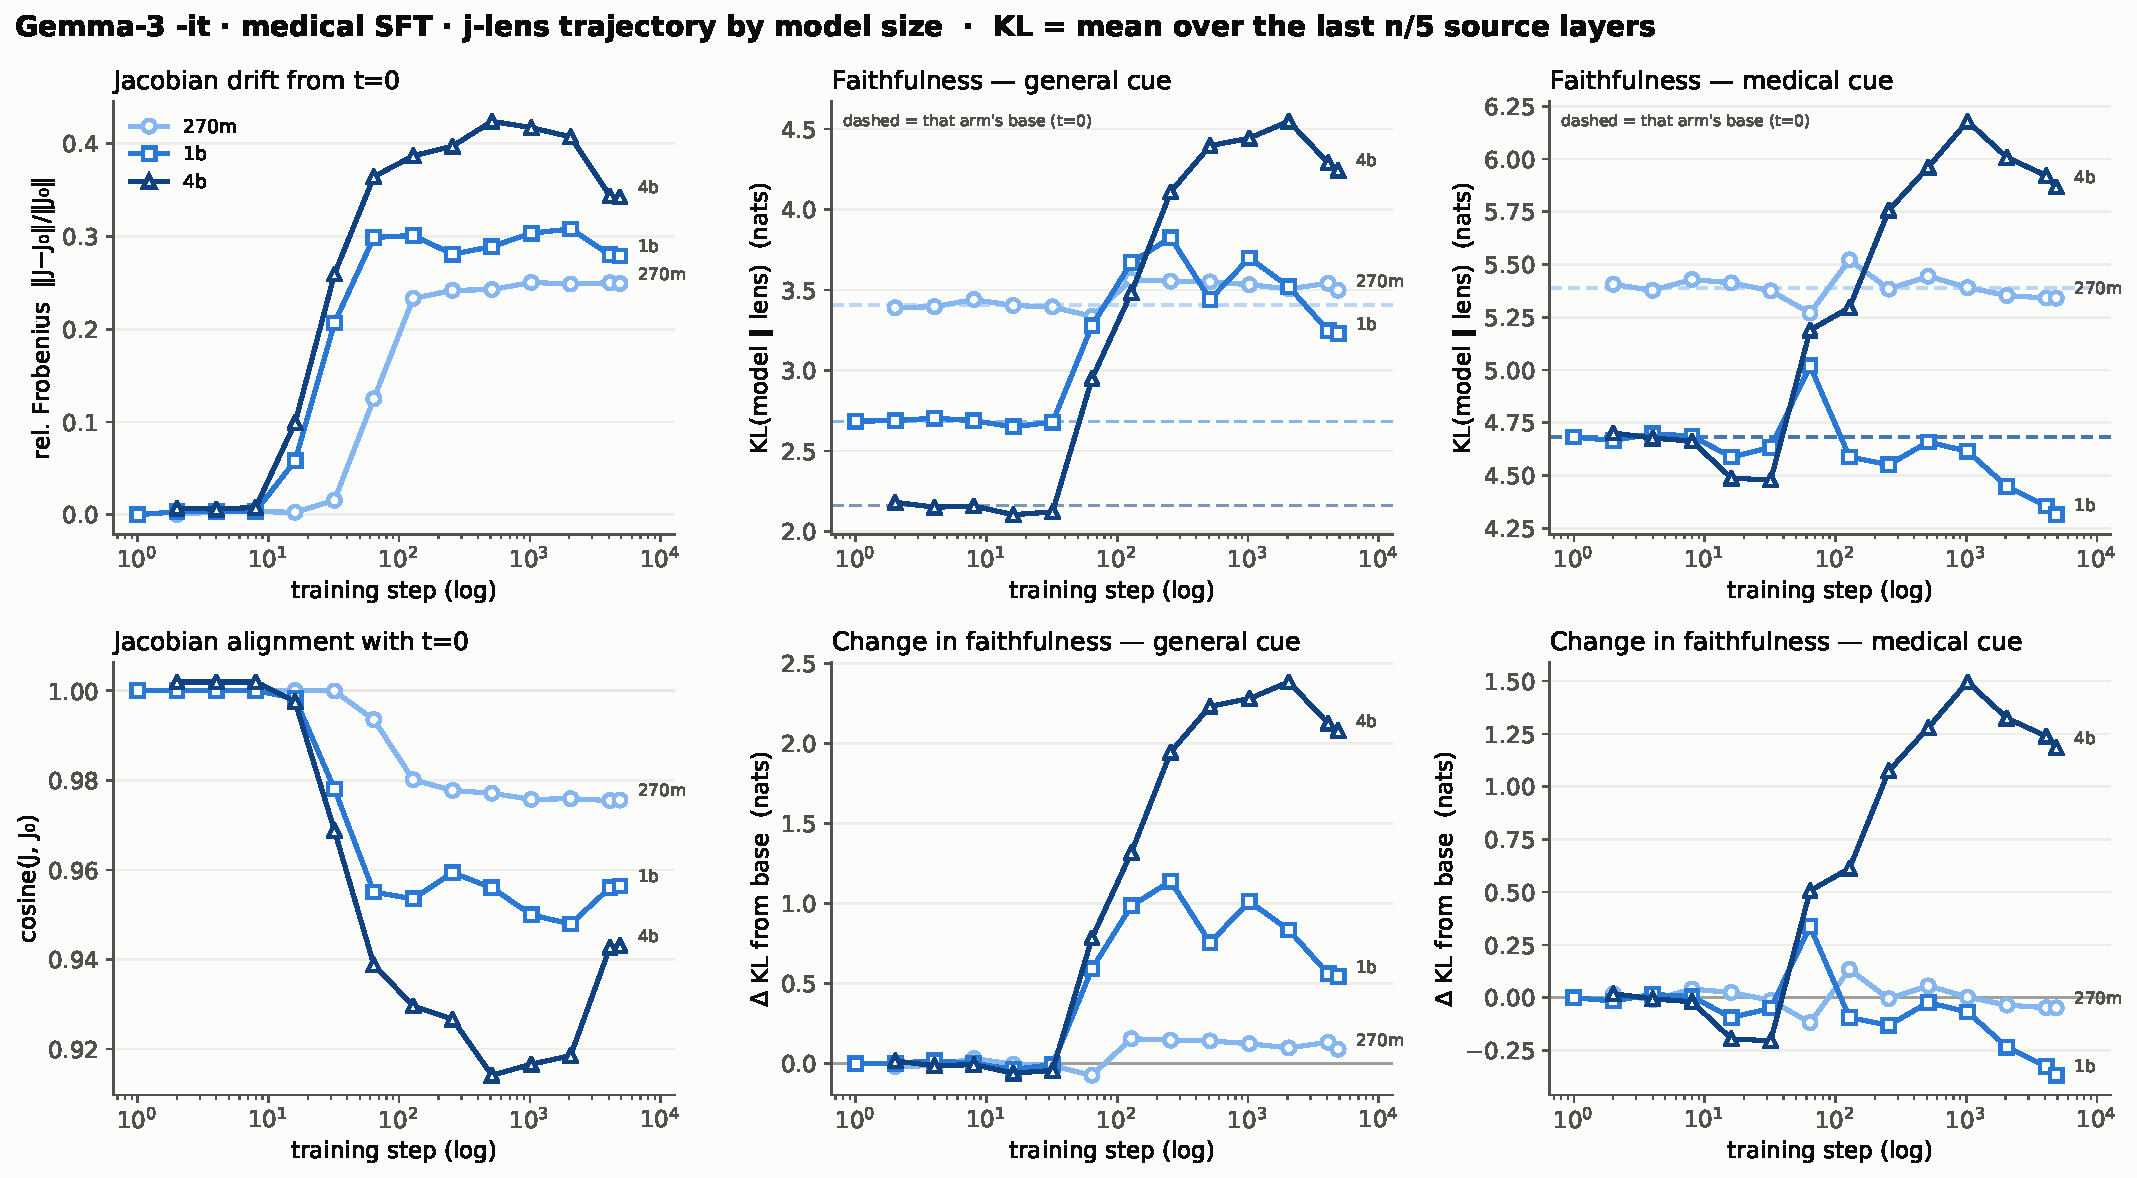
\includegraphics[width=0.82\textwidth]{arms/fig_arms.pdf}

  \vspace{0.1em}
  {\scriptsize Arms shaded light$\rightarrow$dark by size (an \emph{ordinal}
  ramp --- size is ordered, so it does not take categorical hues). $x$ is the
  real training step on a log axis, since the arms have different step grids;
  $t{=}0$ is each arm's dashed baseline (top row) and the zero line (bottom
  row), never a point. \textbf{The bottom-right panel is the held finding}: 12b
  (darkest) runs \emph{below} zero for the whole trajectory while 4b runs above
  it.}
\end{frame}

\begin{frame}{2--3. What survives the 12b arm}
  \small
  Both headline size claims reversed, but the trajectory data are not
  uninformative. One statement holds at \textbf{every} size:

  \vspace{0.7em}
  \centering
  \begin{tabular}{lcccl}
    \toprule
    & $\Delta$ \texttt{medical} & $\Delta$ \texttt{general} & $\Delta$ \texttt{multihop} & medical is\ldots \\
    \midrule
    \texttt{270m-it} & \good{$-0.05$} & \bad{$+0.09$} & \bad{$+0.02$} & least damaged \\
    \texttt{1b-it}   & \good{$-0.37$} & \bad{$+0.54$} & \bad{$+1.01$} & least damaged \\
    \texttt{4b-it}   & \bad{$+1.19$}  & \bad{$+2.08$} & \bad{$+1.63$} & least damaged \\
    \texttt{12b-it}  & \good{$-1.98$} & \bad{$+1.29$} & \bad{$+2.31$} & least damaged \\
    \bottomrule
  \end{tabular}

  \vspace{1.0em}
  \begin{itemize}\setlength{\itemsep}{0.2em}
    \item \good{\textbf{Medical is the least-damaged cue at all four sizes}}
      --- by $0.14$ / $0.91$ / $0.90$ / $3.27$ nats over \texttt{general}. This
      is the finding that has held from two arms to four, and it is
      \emph{directional}, so it does not depend on the cross-size absolute
      comparison the deck forbids.
    \item \textbf{Medical SFT buys the medical cue relative ground at every
      size.} Whether it also buys \emph{absolute} ground is what flips: yes at
      270m/1b/12b, no at 4b.
    \item \bad{Do not read this as ``medical improves.''} At 4b it degrades;
      the claim is only that it degrades \emph{less} than everything else.
  \end{itemize}
  \vfill
  {\footnotesize \good{Read-out check.} Layer mean and single final layer agree
  in sign on all three cues at 4b and 12b. The lone sign flip in this study
  remains 270m \texttt{medical} --- see the read-out caveat.}
\end{frame}

\begin{frame}{2--3. The domain gap narrows at every size --- by three mechanisms}
  \small
  \begin{columns}[T]
    \begin{column}{0.53\textwidth}
      Within each arm the \texttt{medical} cue starts $2$--$4.6$ nats less
      faithful than \texttt{general}. \textbf{All four arms narrow that gap}
      --- but not by the same mechanism.
      \vspace{0.4em}

      \centering
      \begin{tabular}{lcccl}
        \toprule
        & $t{=}0$ & final & $\Delta$ & closes by \\
        \midrule
        \texttt{270m-it} & 1.981 & 1.843 & $-0.138$ & both ends \\
        \texttt{1b-it}   & 1.998 & 1.085 & $-0.912$ & both ends \\
        \texttt{4b-it}   & 2.520 & 1.624 & $-0.895$ & \bad{general only} \\
        \texttt{12b-it}  & 4.625 & 1.355 & $\mathbf{-3.271}$ & both ends \\
        \bottomrule
      \end{tabular}

      \raggedright
      \vspace{0.6em}
      At 270m, 1b and 12b the gap closes \textbf{from both ends} --- medical
      improves \emph{and} general regresses toward it.
      \vspace{0.3em}

      \bad{At 4b it closes from one end}: both cues degrade, \texttt{general}
      just faster ($+2.08$ vs.\ $+1.19$). \textbf{A $-0.9$ gap change means
      opposite things at 1b and 4b} --- which is why the gap is never reported
      on its own.
      \vspace{0.3em}

      12b starts with by far the widest gap ($4.63$) and closes three quarters
      of it. \texttt{multihop} degrades at \emph{all four} sizes
      ($+0.02 / +1.01 / +1.63 / +2.31$).
    \end{column}
    \begin{column}{0.45\textwidth}
      \centering
      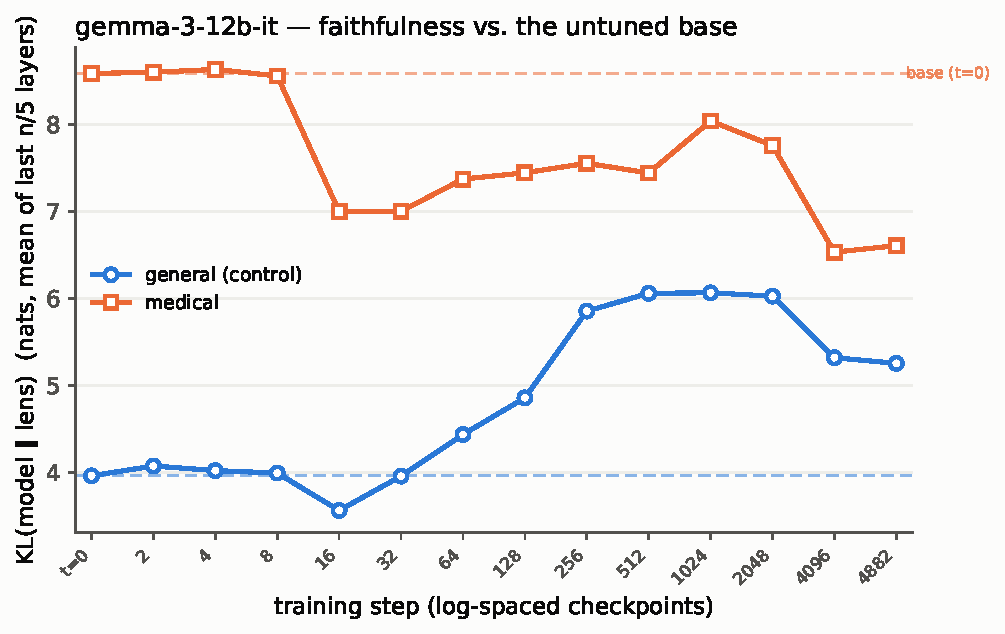
\includegraphics[width=\linewidth]{12b_it_full/fig_kl.pdf}

      \vspace{0.3em}
      {\scriptsize The 12b panel: medical (upper) falls hard toward general
      (lower), which rises --- the ``both ends'' shape. Contrast the 4b panel,
      where both curves rise away from their dashed $t{=}0$ baselines. All four
      arms are on the previous slide.}
    \end{column}
  \end{columns}
\end{frame}

\begin{frame}{2--3. Base vs.\ finetuned, side by side}
  \begin{columns}[T]
    \begin{column}{0.25\textwidth}
      \centering {\small \texttt{270m-it}}\\
      
\includegraphics[width=\linewidth]{270m_it_full/fig_base_vs_final.pdf}
    \end{column}
    \begin{column}{0.25\textwidth}
      \centering {\small \texttt{1b-it}}\\
      
\includegraphics[width=\linewidth]{1b_it_full_v3/fig_base_vs_final.pdf}
    \end{column}
    \begin{column}{0.25\textwidth}
      \centering {\small \texttt{4b-it}}\\
      
\includegraphics[width=\linewidth]{4b_it_full/fig_base_vs_final.pdf}
    \end{column}
    \begin{column}{0.25\textwidth}
      \centering {\small \texttt{12b-it}}\\
      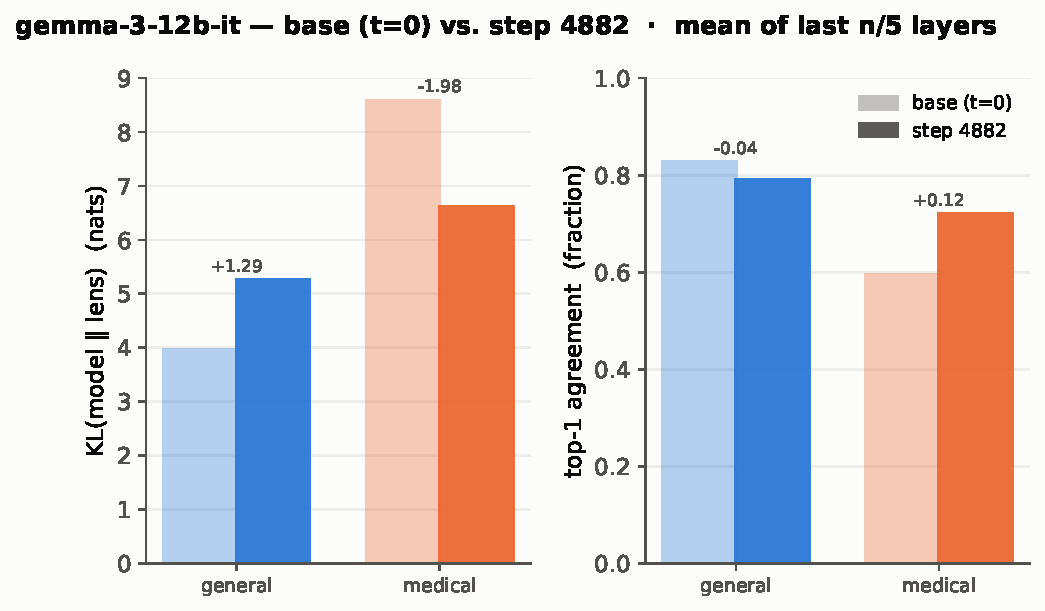
\includegraphics[width=\linewidth]{12b_it_full/fig_base_vs_final.pdf}
    \end{column}
  \end{columns}
  \vspace{0.4em}
  {\footnotesize Pale bar = untuned base ($t{=}0$), solid = step 4882. All four
  are pinned to the same axes (KL $0$--$9$ nats, top-1 $0$--$1$), so the panels
  are directly superimposable --- the range widened from $0$--$6$ to fit 12b's
  medical base at $8.58$.
  Compare the \emph{$\Delta$ labels}, not the bar heights: absolute KL is not
  comparable across sizes (different depth and width, and a different number of
  layers in the $n/5$ mean). Read that way, 270m's largest KL move ($+0.09$) is
  about a quarter of 1b's smallest ($-0.37$), and 12b's medical move ($-1.98$)
  is the largest at any size in either direction.}
\end{frame}

% ---------------------------------------------------------------- behavior
\begin{frame}{4. The instrument, and why every old behavioral number is void}
  \small
  \bad{Two things changed at once on 2026-08-05}, and both invalidate
  comparisons to any earlier version of this deck.

  \vspace{0.4em}
  \begin{columns}[T]
    \begin{column}{0.49\textwidth}
      {\footnotesize
      \textbf{1. Decoding: \texttt{rp}$=$\texttt{1.0} $\rightarrow$
      \texttt{1.1}}
      \begin{itemize}\setlength{\itemsep}{0.2em}
        \item The old answer-rate collapse was \textbf{verbatim repetition
          loops under greedy decoding}, not chain-of-thought overrunning the
          token cap. At 4b step-4882, 311 of 327 unanswered MedMCQA rows were
          loops; 8 were real truncation.
        \item A repetition penalty fixes it outright: 4b MedQA answer rate now
          never leaves $97.9$--$99.8\%$ across the whole trajectory (it
          bottomed at $83.8\%$ before).
        \item \good{No capability appears.} \texttt{acc\_answered} is
          essentially unchanged --- the knowledge was never missing, only the
          format.
      \end{itemize}}
    \end{column}
    \begin{column}{0.49\textwidth}
      {\footnotesize
      \textbf{2. Judge: Claude Haiku $\rightarrow$ self-hosted Kimi}
      \begin{itemize}\setlength{\itemsep}{0.2em}
        \item Scoring is an \textbf{LLM judge} (\texttt{gemma\_med.judge}), not
          a regex: it matches option \emph{content}, not the letter, and is told
          the gold answer and forbidden to re-derive it.
        \item Judge \emph{decode} is now frozen too --- \texttt{temperature=0.0,
          seed=0}, recorded as \texttt{judge\_decode}. Before this date each
          provider sampled at its own default, so ``the judge'' was frozen at
          the model level only.
        \item \good{All four arms are now judge-scored by the same judge},
          which is what makes the cross-size table on the next slide legitimate.
      \end{itemize}}
    \end{column}
  \end{columns}

  \vspace{0.4em}
  {\scriptsize \good{Both changes are cross-validated.} Judge: on 300 identical
  MedQA rows at 4b step-1024, Claude Haiku and Kimi agree to within $1.3$ pp raw
  ($45.0$ vs.\ $46.3$). Judge decode: re-judging the same rows twice flipped
  \texttt{chosen} on $1.34\%$ under the old wire vs.\ $0.33\%$ at $t{=}0$, so the
  old config moved \texttt{acc\_raw} by up to $1.0$ pp \emph{between two
  identical runs}; old-vs-new differs by $\leq 0.67$ pp, i.e.\ inside that
  noise. Freezing buys reproducibility, not a different answer.
  \bad{$t{=}0$ is still not bitwise deterministic} --- batch composition moves
  floating-point ties.}
\end{frame}

\begin{frame}{4. Behavior --- all four arms, one instrument}
  \small
  Judge-scored at \texttt{rp}$=$\texttt{1.1}. \textbf{Answered} accuracy, with
  answer rate in parentheses. $t{=}0$ is each arm's untuned base.

  \vspace{0.5em}
  \centering
  {\footnotesize
  \begin{tabular}{lccc}
    \toprule
    & MedQA & MedMCQA & PubMedQA \\
    \midrule
    \texttt{270m-it} $t{=}0$  & 26.7 \; (96.5\%) & 36.9 \; (\bad{59.3\%}) & 57.8 \; (\bad{21.8\%}) \\
    \texttt{270m-it} final    & 24.8 \; (89.5\%) & 26.6 \; (92.5\%) & 55.0 \; (79.2\%) \\
    \quad $\Delta$            & \bad{$-1.9$} & \bad{$-10.2$} & \bad{$-2.8$} \\
    \addlinespace
    \texttt{1b-it} $t{=}0$    & 31.1 \; (99.9\%) & 34.3 \; (99.9\%) & 51.6 \; (100\%) \\
    \texttt{1b-it} final      & 35.3 \; (99.0\%) & 37.0 \; (99.0\%) & 54.4 \; (99.6\%) \\
    \quad $\Delta$            & \good{$+4.3$} & \good{$+2.7$} & \good{$+2.8$} \\
    \addlinespace
    \texttt{4b-it} $t{=}0$    & 50.9 \; (99.9\%) & 46.6 \; (99.8\%) & 60.0 \; (100\%) \\
    \texttt{4b-it} final      & \good{\textbf{59.2}} \; (99.5\%) & \good{\textbf{53.6}} \; (99.5\%) & \good{\textbf{73.2}} \; (100\%) \\
    \quad $\Delta$            & \good{$+8.2$} & \good{$+7.0$} & \good{$+13.2$} \\
    \addlinespace
    \texttt{12b-it} $t{=}0$   & 70.0 \; (100\%) & 58.8 \; (100\%) & 56.4 \; (100\%) \\
    \texttt{12b-it} final     & \good{\textbf{71.0}} \; (98.8\%) & \good{\textbf{65.0}} \; (99.5\%) & \good{\textbf{78.0}} \; (100\%) \\
    \quad $\Delta$            & \good{$+1.0$} & \good{$+6.2$} & \good{$+21.6$} \\
    \bottomrule
  \end{tabular}}

  \vspace{0.4em}
  {\footnotesize
  \begin{itemize}\setlength{\itemsep}{0.1em}
    \item \bad{\textbf{270m is the only arm that gets worse}} --- and not by
      format churn: its answer rate \emph{improves} on two of three benchmarks
      while answered accuracy falls on all three.
    \item \textbf{The gain is bounded by headroom, not size.} 12b gains $+1.0$
      on MedQA from a base of $70.0$, but $+21.6$ on PubMedQA from $56.4$ ---
      the largest single gain in the study.
  \end{itemize}}
\end{frame}

\begin{frame}{4. A second failure mode: collapse onto the majority label}
  \small
  Format collapse is not the only thing that goes wrong mid-training. Share of
  \emph{answered} items assigned to the dominant label, against that label's
  prevalence in the gold answers:

  \vspace{0.5em}
  \centering
  \begin{tabular}{lcccccc}
    \toprule
    & \multicolumn{2}{c}{MedQA (``A'')} & \multicolumn{2}{c}{MedMCQA (``A'')}
    & \multicolumn{2}{c}{PubMedQA (``yes'')} \\
    \cmidrule(lr){2-3}\cmidrule(lr){4-5}\cmidrule(lr){6-7}
    & chosen & gold & chosen & gold & chosen & gold \\
    \midrule
    $t{=}0$      & 18.5 & 27.7 & 21.6 & 32.2 & 50.4 & 55.2 \\
    step 512     & 28.6 & 27.7 & 37.5 & 32.2 & 65.2 & 55.2 \\
    step 1024    & \bad{\textbf{37.7}} & 27.7 & \bad{\textbf{39.3}} & 32.2 & \bad{69.7} & 55.2 \\
    final        & 29.5 & 27.7 & 33.1 & 32.2 & 66.8 & 55.2 \\
    \bottomrule
  \end{tabular}

  \vspace{0.8em}
  \begin{itemize}\setlength{\itemsep}{0.2em}
    \item \textbf{The base model is \emph{anti}-majority} ($18.5$ vs.\ $27.7$).
      SFT pushes it through neutral and overshoots.
    \item \textbf{Step 1024 is a spike, not a trend} --- it recovers. Worth
      knowing before building a story on any single checkpoint.
    \item \textbf{PubMedQA is the control that reframes it.} It has no ``A'' to
      collapse onto, yet shows the same overshoot on ``yes''. So this is
      \textbf{majority-label over-commitment, not position bias.}
  \end{itemize}
  \vfill
  {\footnotesize \good{This mode survives the instrument change} --- recomputed
  at \texttt{rp}$=$\texttt{1.1}, it is the same shape, roughly two-thirds the
  amplitude (the MedQA step-1024 spike was $57.2$ at \texttt{rp}$=$\texttt{1.0},
  $37.7$ now). \bad{Unlike the format-collapse mode, it is not a decoding
  artifact.} Note this means the two failure modes no longer trade off: with
  format compliance held near $100\%$ throughout, over-commitment is now the
  \emph{only} mid-training pathology visible at 4b.}
\end{frame}

\begin{frame}{4. Joined behavioral + lens trajectory --- \texttt{4b-it}}
  \centering
  
\includegraphics[height=0.78\textheight]{4b_it_full_rp11/fig_joined.pdf}

  {\footnotesize Judge-scored at \texttt{rp}$=$\texttt{1.1}. \bad{Compare this
  against the previous version of the deck:} answer rate (blue) now sits flat
  near the top instead of diverging from answered accuracy (orange) at step 32.
  The format/knowledge split that this panel used to make visible was the
  decoding.}
\end{frame}

\begin{frame}{4. Joined behavioral + lens trajectory --- \texttt{12b-it}}
  \centering
  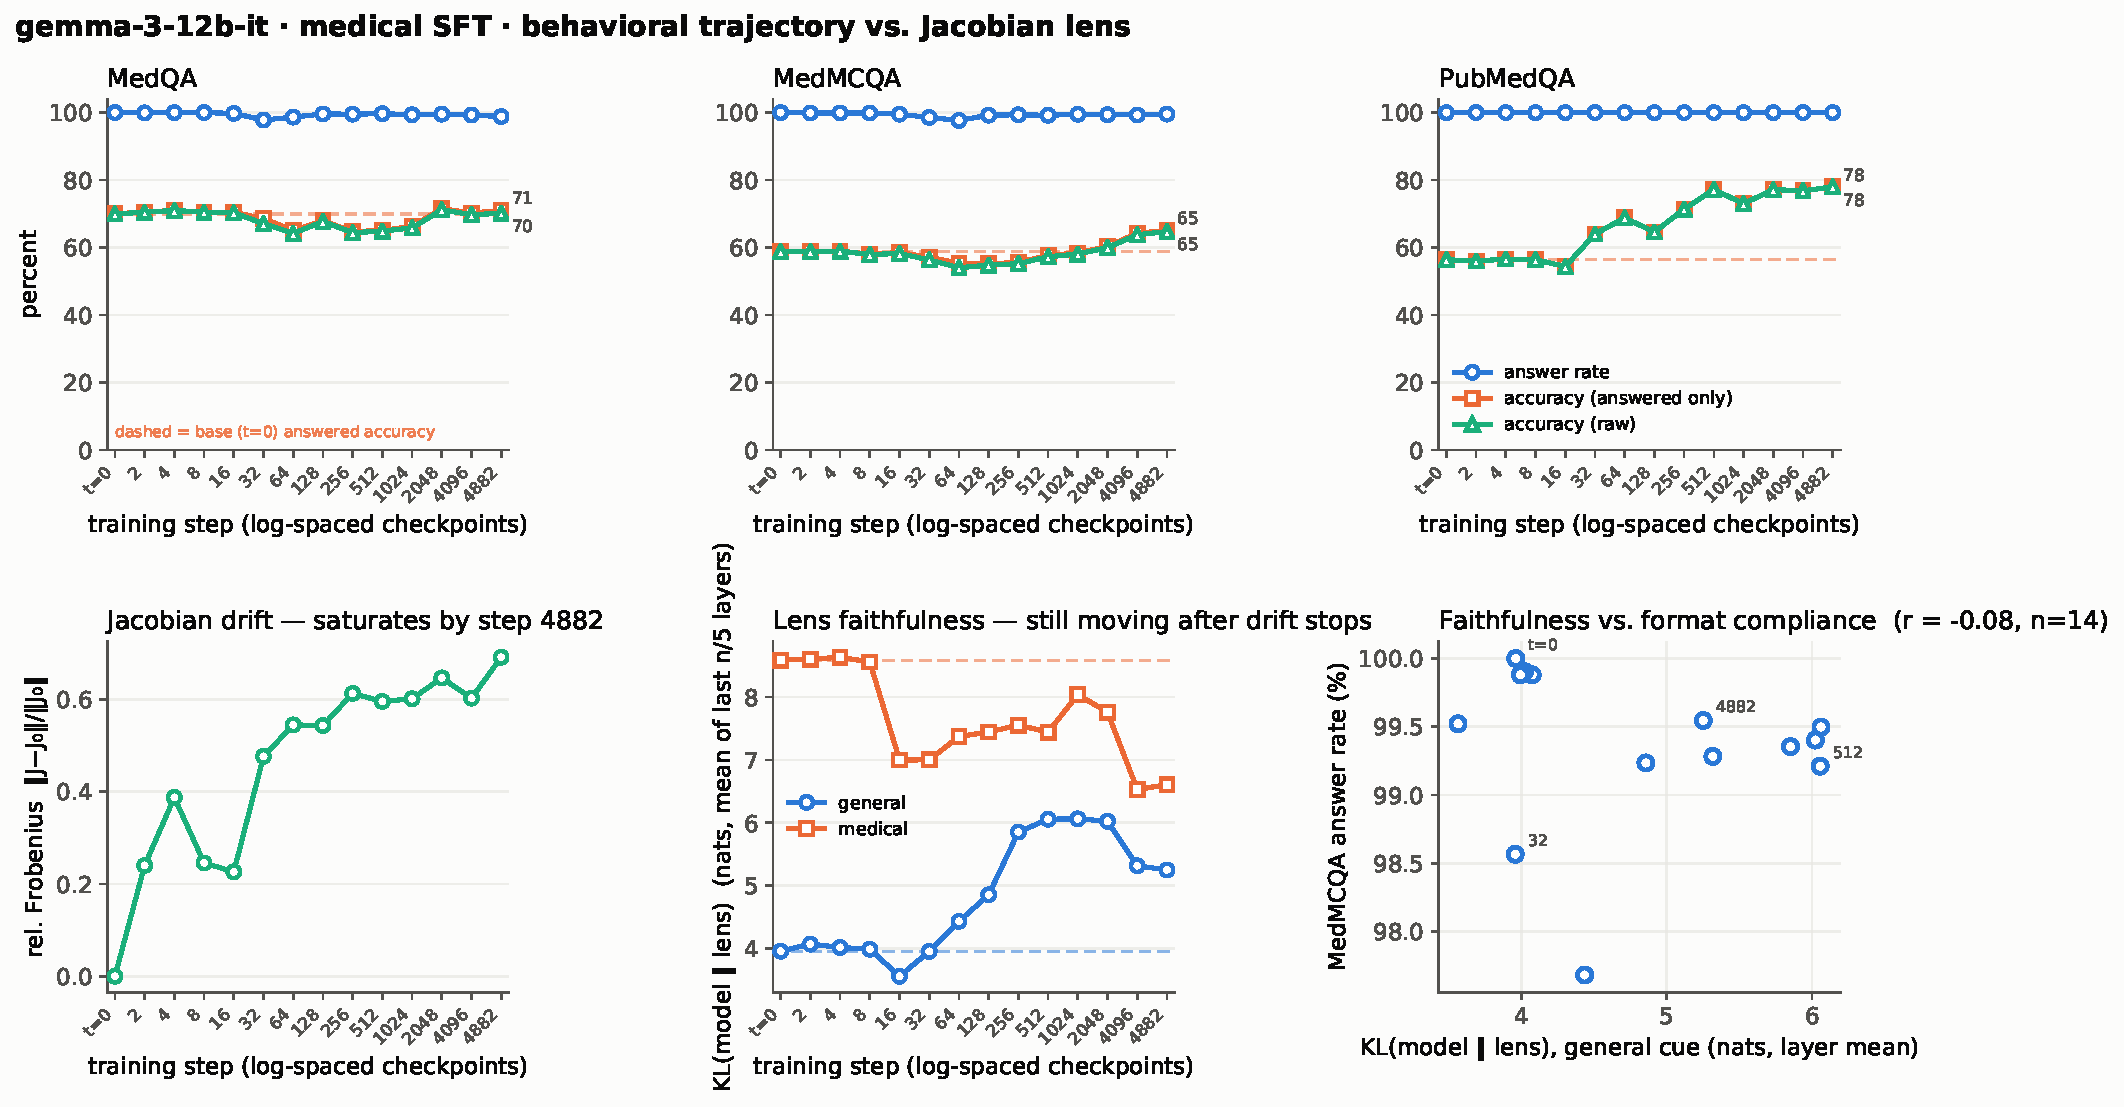
\includegraphics[height=0.80\textheight]{12b_it_full_rp11/fig_joined.pdf}
\end{frame}

\begin{frame}{4. Joined behavioral + lens trajectory --- \texttt{1b-it}}
  \centering
  
\includegraphics[height=0.80\textheight]{1b_it_full_v3_rp11/fig_joined.pdf}
\end{frame}

\begin{frame}{4. Joined behavioral + lens trajectory --- \texttt{270m-it}}
  \centering
  
\includegraphics[height=0.76\textheight]{270m_it_full_rp11/fig_joined.pdf}

  {\footnotesize The KL panel is the layer mean, as everywhere else in this
  deck; at the single final layer the medical curve rises instead. 270m is the
  one arm where answer rate still moves a lot under \texttt{rp}$=$\texttt{1.1}
  --- it \emph{rises} (MedMCQA $59 \rightarrow 92\%$), which is why its
  drift$\leftrightarrow$rate correlation comes out \emph{positive}.}
\end{frame}

% ---------------------------------------------------------------- timing
\begin{frame}{5. Timing holds; the correlation behind it does not}
  \small
  \textbf{The ordering is the robust part}, and it holds at all four sizes ---
  \texttt{4b-it} shown:

  \vspace{0.4em}
  \centering
  {\footnotesize
  \begin{tabular}{lll}
    \toprule
    Signal & Onset & Notes \\
    \midrule
    Jacobian drift      & steps 16--32  & $0.099 \rightarrow 0.259$ (layer mean); plateaus by step 64 \\
    Task accuracy       & steps 2048+   & MedQA answered $52.6$ at step 512; $59$ only at 2048--4882 \\
    \bottomrule
  \end{tabular}}

  \vspace{0.8em}
  \bad{\textbf{But ``drift leads format collapse'' does not survive
  \texttt{rp}$=$\texttt{1.1}}} --- Pearson $r$ vs.\ drift (layer mean),
  answer rate / answered accuracy:

  \vspace{0.3em}
  \centering
  {\footnotesize
  \begin{tabular}{lccc}
    \toprule
    & MedQA & MedMCQA & PubMedQA \\
    \midrule
    \texttt{270m-it} & $-0.49$ / $-0.22$ & \bad{$\mathbf{+0.92}$} / $-0.99$ & $+0.97$ / $-0.56$ \\
    \texttt{1b-it}   & $-0.33$ / $+0.11$ & $-0.20$ / $+0.05$ & $-0.31$ / $+0.73$ \\
    \texttt{4b-it}   & $-0.47$ / $+0.06$ & $-0.65$ / $+0.15$ & $-0.27$ / $+0.57$ \\
    \texttt{12b-it}  & $-0.48$ / $-0.49$ & $-0.48$ / $+0.07$ & --- / $+0.90$ \\
    \bottomrule
  \end{tabular}}

  \vspace{0.5em}
  {\footnotesize
  \begin{itemize}\setlength{\itemsep}{0.1em}
    \item The old $\mathbf{-0.91}$ on 4b MedMCQA is now $-0.65$, and the sign
      \bad{flips outright at 270m} ($+0.92$) --- there answer rate \emph{rises}
      over training. (PubMedQA at 12b is \texttt{---}: answer rate is exactly
      $100.0\%$ at every checkpoint, so $r$ is undefined.)
    \item \textbf{With format compliance pinned near $100\%$ by the decoding,
      there is almost no variance in answer rate left to correlate with.} The
      old $r$ was measuring an artifact of greedy decoding.
    \item \textbf{What still stands:} the Jacobian finishes moving before the
      model learns any medicine. \bad{What does not:} that it moves \emph{with}
      format collapse specifically.
  \end{itemize}}
\end{frame}

% ---------------------------------------------------------------- caveats
\begin{frame}{Caveats --- the measurements}
  \small
  \begin{itemize}\setlength{\itemsep}{0.5em}
    \item \textbf{Top-1 is coarse.} $n{=}50$ prompts for
      \texttt{general}/\texttt{medical} ($93$ for \texttt{multihop}), so
      \emph{per-layer} top-1 quantizes at $0.02$; the reported statistic
      averages 3 / 5 / 6 / 9 layers, giving a $1/150$--$1/450$ grain that
      makes small moves look more precise than they are. Single-checkpoint
      wiggles of $\pm 0.04$ are still noise. \emph{Trust the KL trends, not
      top-1.}
    \item \textbf{Read-out choice is not innocent.} Layer-mean and final-layer
      KL disagree in sign on 270m medical. Every claim here uses the layer mean;
      an earlier draft of this deck used the final layer and reported a
      270m$\leftrightarrow$1b \emph{inversion} that does not survive. Report the
      statistic, not just the number. \good{(It does not recur at 4b.)}
    \item \textbf{A numerical artifact in the drift cosine.} At 4b steps 2--8,
      \texttt{cos\_mean} reads $1.001$--$1.003$; cosine cannot exceed 1. The
      fp32 \texttt{dot} over ${\sim}6.5$M entries per layer is biased against
      the stabler norm computation. Only visible where drift ${\approx}0$; no
      reported claim depends on it, but \texttt{jac\_drift} should accumulate
      in fp64.
    \item \textbf{The \texttt{general}/\texttt{medical} cues are
      hand-authored}, not sampled from a corpus --- the domain-gap result
      inherits whatever bias is in those 100 prompts. \texttt{multihop} is the
      one cue with an external, independently-constructed source.
  \end{itemize}
\end{frame}

\begin{frame}{Caveats --- the scope}
  \small
  \begin{itemize}\setlength{\itemsep}{0.7em}
    \item \bad{\textbf{Four sizes is still not a scaling curve.}} The 12b arm
      did not extend the trend it was run to test --- it reversed it, on both
      \texttt{general} and \texttt{medical}. Four points spanning ${\sim}44\times$
      in parameters now show one non-monotone cue, one monotone cue, and a
      medical cue whose sign alternates. \textbf{27b arbitrates 4b-vs-12b but
      cannot make four noisy points into a curve.}
    \item \bad{\textbf{One hyperparameter setting --- now the load-bearing
      caveat.}} All four arms are full FT at lr $1\mathrm{e}{-5}$ on one
      mixture. Whether these deltas are about \emph{size}, or about a fixed LR
      being progressively too large as the model grows, is not separable from
      these runs --- and \textbf{a non-monotone \texttt{general} curve is
      exactly that confound's signature}. The decisive experiment is a second
      LR at one size, not a fifth size.
    \item \good{\textbf{The behavioral instrument is finally uniform}} --- four
      arms, one decode config, one judge, judged $t{=}0$ baselines for all.
      Cross-size behavioral comparison is legitimate for the first time.
      \bad{The cost:} every behavioral number predating 2026-08-05 is void, and
      finding 5 did not survive the change.
    \item \textbf{Coverage gaps.} 4b, 270m and 12b have no
      \texttt{checkpoint-1}, so their grids start at step 2; only 1b probed
      step 1. No \texttt{-pt} arm exists at any size --- the pt-vs-it
      starting-point axis is entirely unstarted.
    \item \textbf{The 12b early-step drift is unexplained.} $0.055$ at step 2
      against ${\leq}0.008$ for the three smaller arms. Real early motion or a
      noisier fit at $d_\text{model}{=}3840$ --- not yet distinguished, and it
      is the one number in finding 1 that is provisional.
  \end{itemize}
\end{frame}

% ---------------------------------------------------------------- next
\begin{frame}{Next}
  \begin{enumerate}\setlength{\itemsep}{0.3em}
    \item \textbf{Finish 27b} and settle findings 2--3. The behavioral half is
      already decoded and judged at both \texttt{rp} values; the lens is 8/13
      checkpoints in, at ${\sim}34$\,h per checkpoint. \textbf{This is the only
      blocker on un-holding the two findings.}
    \item \bad{\textbf{A second LR at one size}} --- 4b or 12b at, say,
      $3\mathrm{e}{-6}$. Now the highest-value experiment in the study: it is
      the only thing that separates ``the cost is about size'' from ``the cost
      is about a fixed LR being too large for a bigger model,'' and the 12b
      reversal is what makes that ambiguity load-bearing rather than pedantic.
    \item \textbf{Widen the \texttt{general}/\texttt{medical} cues} beyond the
      100 hand-authored prompts, to check the domain-gap collapse is not an
      artifact of how those pairs were written. 12b's $4.63$-nat starting gap
      makes this more pressing, not less.
    \item \textbf{Open a \texttt{-pt} arm} at 1b: does a non-aligned starting
      point show the same drift-before-competence ordering?
    \item \textbf{Anchor against \texttt{medgemma-27b-text-it}} on the same
      probe set to place the trajectory endpoints on an absolute scale.
  \end{enumerate}
  \vfill
  {\footnotesize Answered since the last version: \textbf{270m and 1b are
  re-judged}, so all four arms share one instrument; \textbf{the 12b arm exists}
  end to end. \bad{Retracted since the last version:} the size-monotone
  faithfulness cost (finding 2), medical-is-not-protected (finding 3), and
  drift-leads-format-collapse at $r=-0.91$ (finding 5) --- the first two by 12b,
  the third by the decode fix.}
\end{frame}

\begin{frame}{Data provenance}
  \small
  \begin{tabular}{ll}
    \toprule
    Artifact & Path \\
    \midrule
    Lens metrics & \texttt{eval/jlens/\{270m\_it\_full, 1b\_it\_full\_v3,} \\
                 & \texttt{4b\_it\_full, 12b\_it\_full\}/metrics.jsonl} (14/15/14/14 rows) \\
    Joined traj. & \texttt{eval/traj/<arm>\_rp11/joined.json} \good{(all judge-scored)} \\
    $t{=}0$ dirs & \texttt{eval/gemma-3-\{270m,1b,4b,12b\}-it-baseline-rp11/} \\
    Fit corpus   & \texttt{data/jlens/fit\_corpus\_v2.txt} (1000 WikiText seq, frozen) \\
    Probe set    & \texttt{data/jlens/probe\_set\_v2.tsv} (50/50/93, frozen) \\
    Figures      & \texttt{figs/<lens-tag>/} lens (decode-independent); \\
                 & \texttt{figs/<arm>\_rp11/fig\_joined.pdf} (decode-dependent) \\
    Probe jobs   & \texttt{25776556} (1b), \texttt{25799677} (270m), \\
                 & \texttt{25948088--25948100} (4b), 13-way fanout (12b) \\
    \bottomrule
  \end{tabular}

  \vspace{0.4em}
  {\scriptsize All four runs logged \texttt{fit\_corpus=1000 probes=193} --- the
  frozen v2 inputs. The v1 files (40 seq / 30 prompts) are legacy, still in
  \texttt{data/jlens/}, used only by the superseded runs.

  \smallskip
  \textbf{4b and 12b were probed one Slurm job per checkpoint} (4b ${\sim}3.5$\,h
  each; 12b longer --- fit cost scales as $d_\text{model} \times$ params), all 13
  workers reusing the \emph{same} fp32 $t{=}0$ lens so drift shares one baseline;
  rows merged by \texttt{scripts/merge\_jlens\_fanout.py}, which refuses the
  merge if any non-base step appears twice.

  \smallskip
  Superseded: \texttt{4b\_it\_validate\{,2\}} (wrapper-validation spikes),
  \texttt{1b\_it\_full\_v2} (v1 30-prompt set), \texttt{1b\_it\_full\_probev2},
  \texttt{270m\_verify} (Phase-0 smoke test).}
\end{frame}

\begin{frame}{Data provenance --- the behavioral instrument (all four arms)}
  \small
  \begin{tabular}{ll}
    \toprule
    Field & Value \\
    \midrule
    Decode     & \texttt{temperature=0.0, max\_new\_tokens=1024,} \\
               & \texttt{repetition\_penalty=1.1, seed=0} \; \textbf{frozen 2026-08-05} \\
    Scorer     & \texttt{gemma\_med.judge} (replaces \texttt{answer\_parsing.py}) \\
    Provider   & \texttt{local} --- the lab's self-hosted Kimi, BigPurple only \\
    Judge model& \texttt{Barney} \; \textbf{frozen for all four trajectories} \\
    Judge decode& \texttt{temperature=0.0, seed=0} \; \textbf{also frozen 2026-08-05} \\
    Verdicts   & \texttt{correct} / \texttt{incorrect} / \texttt{no\_answer},
                 schema-constrained \\
    Judgments  & \texttt{eval/traj/*\_rp11/step-*/*\_judgments.jsonl} \\
    Provenance & \texttt{.../step-*/judged\_summary.json} (13/14/13/13 files) \\
    \bottomrule
  \end{tabular}

  \vspace{0.6em}
  {\scriptsize
  \textbf{A second decode is on disk and must not be mixed in.} Every arm was
  also decoded at \texttt{rp}$=$\texttt{1.05} (\texttt{eval/traj/*\_rp105/}),
  kept as a sensitivity check: it halves the repetition loops while costing less
  \texttt{acc\_answered} than $1.10$ does, and it preserves a muted version of
  the old answer-rate dip (4b MedQA $92.9\%$ at step 512 vs.\ $97.9\%$ at
  \texttt{rp}$=$\texttt{1.1}). \bad{Different instrument --- never in the same
  figure.}

  \smallskip
  \textbf{\texttt{judge\_self\_disagreement} --- a quality signal that scores
  nothing.} It counts rows where the judge's verdict string conflicts with the
  option it picked: $0.05$--$0.25\%$ on these runs. \good{It changes no number}
  --- \texttt{correct} and \texttt{answered} are both recomputed from
  \texttt{chosen}, never from \texttt{verdict}. It ran higher
  ($0.95\%$ overall, peaking $2.8\%$) on the \texttt{rp}$=$\texttt{1.0} corpus,
  where the judged model rambled more; the statistic tracks \textbf{how rambly
  the judged model is}, not how confused the judge is.}
\end{frame}

\end{document}
